\subsection{Mechanism flowchart}
All formulas and theories are established for 2D, 3D, and kD-Laplace, so the mechanism design applies to all three variants:
\begin{figure}[H]
    \includesvg[width=1\textwidth]{TheorethicalFramework/ND-Laplace/Images/final_mechanism_design}
    \caption{Non-interactive mechanism design for kD-Laplace.}
    \label{fig:final-mechanism-design}
\end{figure}
For easy navigation, we provide a list of all algorithms \todo[inline]{Modify to density-kD-Laplace \& kD-Laplace for image reporting}:
\begin{enumerate}
    \item 2D-Laplace:  \ref{alg:2d-laplace}
    \item 3D-Laplace: \ref{alg:3d-laplace}
    \item kD-Laplace: \ref{alg:nd-laplace}
    \item Find points outside domain: \ref{alg:find-outside-domain-laplace}
    \item Grid remapping: \ref{alg:grid-remapping-laplace}
    \item Distance remapping: \ref{alg:optimal-remapping-laplace}
\end{enumerate}
\subsubsection{Practical example}
The shape of the dataset is necessary for the usefulness of clustering.
With our algorithm, there are four different shapes/variants of the dataset.
For example, this has been visualized using a 3D dataset based on the heart dataset (\ref{datasets-section}).
Our mechanism aims to provide privacy and preserve the dataset's shape to benefit the utility of clustering.
Grid remapping and optimal remapping are used to achieve this goal.

\begin{figure}[H]
    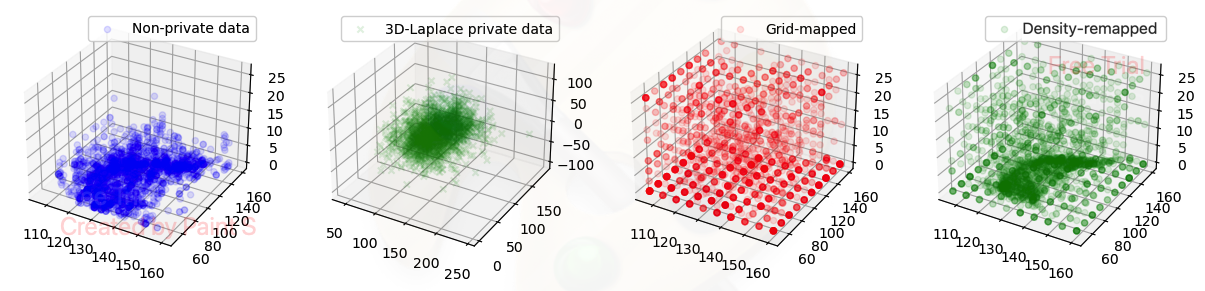
\includegraphics[width=1.1\textwidth]{TheorethicalFramework/ND-Laplace/Images/optimal-remapping-example.png}
    \caption{Example of optimal remapping for the 3D-dataset: Cardiotocography. The example shows the different steps of the mechanism in sequence for a dataset perturbed with a privacy budget of 0.1.}
\end{figure}

\begin{enumerate}
    \item Dataset: the blue dots represent the original dataset without any modifications.
    \item Adding noise: the green crosses represent the dataset after adding noise; for this particular example, this is 3D-Laplace (Algorithm \ref{alg:3d-laplace}):
          As can be observed, the data is generated from the center, causing many data points to fall outside the original domain of the dataset.
    \item Grid-remapping: the red dots represent the dataset after grid-remapping (Algorithm \ref{alg:grid-remapping-laplace})
          After performing the grid remapping algorithm, all points within the domain are plotted.
          However, the original shape of the data is mostly lost.
          This makes it challenging to cluster the data as was possible with the original data.
    \item Optimal-remapping: the green dots represent the dataset after optimal-remapping (Algorithm \ref{alg:optimal-remapping-laplace}).
          After completing the previous step, the data points are again remapped based on the (original) density.
          This results in restoring the original shape of the data and, consequently, the clusters.
\end{enumerate}
